\subsubsection{Przygotowanie}
Wszystkie przygotowane skrypty testowe rozpoczynają się od przygotowania środowiska do~trenowania modelu.
Najpierw ustawiana jest ścieżka do~katalogów z~wygenerowanymi grafami oraz do~katalogów na~dane treningowe i~walidacyjne.
Następnie sprawdzane jest, czy te katalogi istnieją, a~jeśli nie, są tworzone.
Dalej, skrypty definiują parametry dotyczące wielkości obrazów oraz wielkości partii danych, które będą używane podczas treningu.
Dla każdej wartości liczby wierzchołków ustawiana jest ścieżka do~katalogu z~wygenerowanymi grafami,
pobierana lista podkatalogów oraz obrazów w~każdym z~nich.
Następnie obrazy dzielone są na~zestawy treningowe i~walidacyjne w~stosunku 80:20.
Daje to~8 tys. grafów w~zbiorze uczącym i~2 tys. grafów w~zbiorze testowym.
W~przypadku modeli wykorzystujących wszystkie warianty liczby wierzchołków, dane przenoszone są do~jednego katalogu
i~od razu dzielone na~zbiory treningowe i~walidacyjne.

\subsubsection{Model}
Każdy typ modelu tworzony jest w~inny sposób. Opisana zostanie tu główna zasada i~ich elementy wspólne.
Na początku, skrypt wczytuje obrazy przygotowane na~wcześniejszym etapie do~odpowiednich zmiennych - treningowe i~walidacyjne.
W~przypadku modeli z~walidacją krzyżową, dla każdej itreacji walidacyjnej, dane zostały podzielone inaczej.
Po wczytaniu danych, zostają one przeskalowane do~wielkości 180x180 pikseli i~przekształcone do~odcieni szarości.

\clearpage

\begin{lstlisting}[language=Python,caption=Listing skryptu tworzącego model z~walidacją krzyżową
	oraz uczonym na~wszystkich wariantach liczby wierzchołków grafów,label={tests-model-1}]
	n_splits = 5
	kfold = KFold(n_splits=n_splits, shuffle=True, random_state=42)
	history = []
	all_images = [os.path.join(dp, f) for dp, dn, filenames in os.walk(data_dir_model) for f in filenames if os.path.splitext(f)[1] == '.png']
  
	for train_index, val_index in kfold.split(all_images):
		train_images = [all_images[i] for i~in train_index]
		validation_images = [all_images[i] for i~in val_index]

		# Generowanie danych treningowych
		train_ds = tf.keras.preprocessing.image_dataset_from_directory(
		train_dir,
		image_size=(img_height, img_width),
		batch_size=batch_size)

		class_names = train_ds.class_names

		train_ds = train_ds.map(lambda x, y: (rgb_to_grayscale(x), y))

		# Generowanie danych walidacyjnych
		val_ds = tf.keras.preprocessing.image_dataset_from_directory(
		validation_dir,
		image_size=(img_height, img_width),
		batch_size=batch_size)

		val_ds = val_ds.map(lambda x, y: (rgb_to_grayscale(x), y))

		# Tworzenie modelu
		model = tf.keras.models.Sequential([
		tf.keras.layers.Rescaling(1./255),
		tf.keras.layers.Conv2D(32, 3, activation='relu'),
		tf.keras.layers.MaxPooling2D(),
		tf.keras.layers.Conv2D(32, 3, activation='relu'),
		tf.keras.layers.MaxPooling2D(),
		tf.keras.layers.Conv2D(32, 3, activation='relu'),
		tf.keras.layers.MaxPooling2D(),
		tf.keras.layers.Flatten(),
		tf.keras.layers.Dense(128, activation='relu', kernel_regularizer=tf.keras.regularizers.l2(0.01)),
		tf.keras.layers.Dropout(0.2),
		tf.keras.layers.Dense(len(class_names))
		])
		
		# Kompilacja modelu
		model.compile(
			optimizer='adam',
			loss=tf.losses.SparseCategoricalCrossentropy(from_logits=True),
			metrics=['accuracy']
		)

		# Uczenie modelu
		history.append(model.fit(
			train_ds,
			validation_data=val_ds,
			epochs=75
		))
\end{lstlisting}

Model sieci neuronowej został zdefiniowany jako sekwencyjny stos warstw.
Dla standaryzacji danego testu, w~przypadku modeli z~walidacją krzyżową, ustalono $k$-Fold z~liczbą podziałów równą 5.
Pierwsza warstwa to~warstwa Rescaling, która normalizuje wartości pikseli do~zakresu [0, 1].
W~przykładzie, parametr $1./255$ oznacza, że każda wartość piksela mnożona jest przez $\frac{1}{255}$.
Następne trzy warstwy to~Conv2D, z~których każda jest następowana warstwą MaxPooling2D.
W~przykładzie, warstwa kolwolucyjna stosuje 32 filtry o~wymiarach 3x3 oraz funkcję aktywacji ReLU,
która wprowadza nieliniowość do~modelu.
MaxPooling2D redukuje rozmiar danych wejściowych,
wybierając maksymalną wartość z~każdego regionu (domyślnie oraz tutaj - 2x2). 
Po wyżej wymienionych warstwach, znajduje się warstwa Flatten, która przekształca mapy cech 2D w~wektor 1D.
Innymi słowy, przekształca wielowymiarową macierz wyjściową z~poprzedniej warstwy do~jednowymiarowego wektora.
Następnie, dodana jest w~pełni połączona (Dense) warstwa z~128 neuronami
i~funkcją aktywacji, podobnie jak w~przypadku Conv2D, ReLU.
Wprowadzona jest również regularyzacja L2, która dodaje karę za duże wartości wag,
by zmniejszyć ryzyko przeuczenia. Została zastosowana z~siłą 0,01.
Kolejna warstwa to~Droput, która losowo wyłącza 20\% neuronów podczas uczenia,
co~również jest moetodą zapobiegającą przeuczeniu.
Warstwa wyjściowa zawiera tyle jednostek, ile występuje klas w~danych uczących.
Zależnie od danego testu, może być to~różna liczba.
W~przypadku warstw konwolucyjnych, wybrano 32 filtry, a~dla warstwy w~pełni połączonej zastosowano 128 jednostek.
Liczba epok w~podstawowej wersji modelu wyniosła 75.

W~kolejnych wariantach modeli, zmieniane były parametry poszczególnych warstw, funkcje aktywacji,
czy również same warstwy, w~celu znalezienia najbardziej optymalnej kombinacji.

\subsubsection{Wyniki}
Po wytrenowaniu modelu, skrypt dokonuje wizualizacji dokładności i~straty modelu.
Najpierw wyświetla w~konsoli wartości dokładności dla obu zbiorów z~historii treningu.
Dalej tworzy wykresy, gdzie na~pierwszym z~nich pokazuje dokładność na~zbiorze treningowym i~walidacyjnym,
a~na~drugim wykresie prezentuje stratę modelu dla obu zbiorów.
Jednostką straty jest entropia krzyżowa (cross-entropy), która jest wyrażana jako liczba bezwzględna.
Entropia krzyżowa mierzy różnicę między rzeczywistymi etykietami a~przewidywanymi prawdopodobieństwami klas.
Im mniejsza wartość entropii krzyżowej, tym lepiej model przewiduje klasy.
Dokładność jest wyrażana jako wartość procentowa lub~ułamek, gdzie 1 oznacza 100\% dokładności.
Na przykład, jeśli model przewiduje poprawnie 90 na~100 przypadków, dokładność wynosi 0.9 lub~90\%.

\begin{figure}[ht]
	\centering
	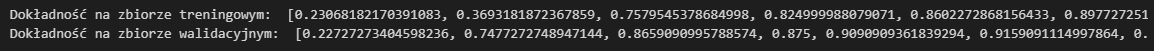
\includegraphics[width=15.5cm]{resources/model/images/scr-standard-result.png}
	\caption{Przykładowe wartości dokładności dla zbioru treningowe i~walidacyjnego}
	\label{Fig:tests-wyniki-2}
\end{figure}
\FloatBarrier

\begin{figure}[ht]
	\centering
	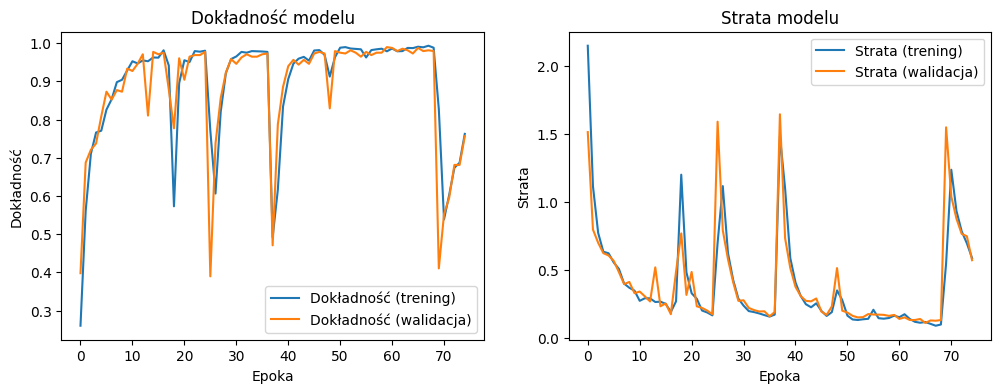
\includegraphics[height=6cm]{resources/model/images/v2_epoch75.png}
	\caption{Przykładowa wizualizacja dokładności i~straty wytrenowanego modelu}
	\label{Fig:tests-wyniki-1}
\end{figure}
\FloatBarrier

\subsubsection{Testy na~danych zewnętrznych}
Po wyświetleniu dokładnosci modelu skrypt przeszukuje katalog z~danymi i~jego podkatalogi, by przygotować obrazy zewnętrzne.
Następnie ustawia ścieżkę do~katalogu z~obrazami testowymi i~pobiera ich listę.
Dla każdego obrazu w~tej liście wczytuje go, przeskalowuje do~odpowiedniego rozmiaru i~konwertuje do~skali szarości
Następnie model przewiduje klasę obrazu, a~wynik jest wyświetlany w~konsoli.